\chapter{Formalismen}
\label{ch:formalism}
In dit hoofdstuk wordt er gekeken naar formalisme binnen interactive story telling. Er wordt een voorstel gedaan op de softwarearchitectuur van de nieuwe editor om meerdere formalisme te ondersteunen in één omgeving. Deze softwarearchitectuur betreft het leggen van een scheiding tussen de editor en het achterliggende formalisme. Het ondersteunen van meerdere formalismen maakt het onderhouden van twee aparte editors overbodig.

\section{Formalismen binnen interactive story telling}
\subsection{De rol van formalisme}
Het formaliseren van het narratief speelt een grote rol tijdens het ontwikkelproces van narrative games. Volgens een vastgesteld formalisme wordt er betekenis gegeven aan de structuur achter het narratief. Een formalisme is een theorie die bepaalde richtlijnen afdwingt maar hier verder geen waarde aankoppelt. In \autoref{fig:simplestorytree} is een voorbeeld van een formalisme terug te zien. Dit formalisme wordt ook wel een story graph genoemd.

Een formalisme dient als een communicatiemiddel tussen zowel mens als computer. Mensen en computers die kennis hebben van het formalisme interpreteren deze vrijwel hetzelfde. Hierdoor kunnen teamleden efficiënt samenwerken aan een narratief; ze zitten op dezelfde lijn en structureren beide volgens het formalisme.

\subsection{Formalismen voor verschillende doeleinden}
\subsubsection{Story graphs}

Veel interactieve verhalen met vertakkingen kunnen worden gerepresenteerd als een boom\cite{GalyeanIII1995}. Deze bestaat uit nodes (ook wel vertices genoemd) die de uiting van de gesprekspartner representeren. Na de evaluatie van deze nodes kan er een keuze gemaakt worden. Deze discrete set van keuzes zijn terug te zien in de story tree als edges, hetgeen dat de nodes met elkaar verbindt. De gemaakte keuze bepaald de volgende node die geëvalueerd zal worden en dus de uitkomst van het verhaal. Dit formalisme laat ons toe om een inzichtelijk en simpele dialoog tussen twee personen te modelleren (\autoref{fig:simplestorytree}).

\begin{figure}[H]
    \centering    
    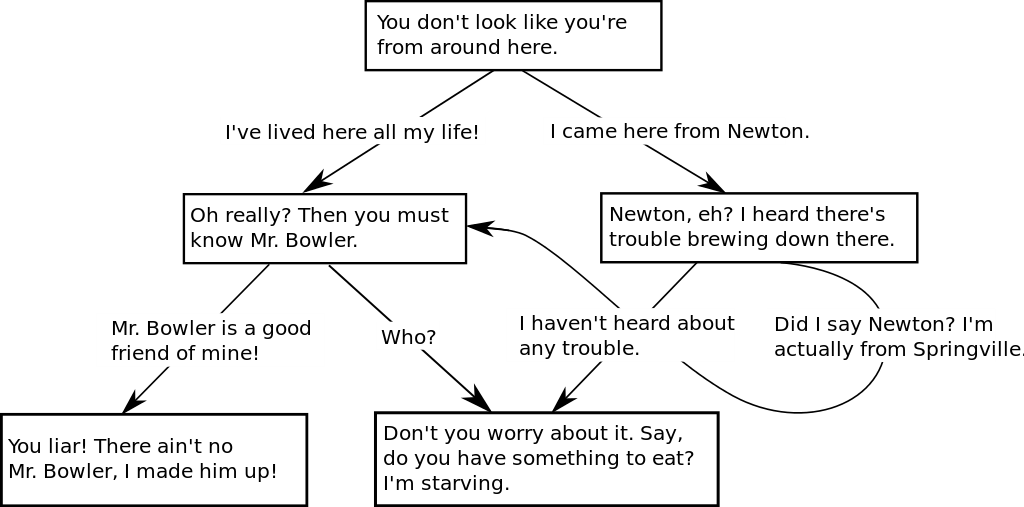
\includegraphics[width=0.95\textwidth]{SimpleStoryTree}
    \caption[]{Een simpele story tree. \footnotemark}
    \label{fig:simplestorytree}
\end{figure}
\footnotetext{Bron: \url{https://commons.wikimedia.org/wiki/File:Dialog_tree_example.svg}}

\subsubsection{Behaviour tree}
// todo

\subsection{Syntactische vormen}

\begin{wrapfigure}{r}{0.4\textwidth}
    \centering    
    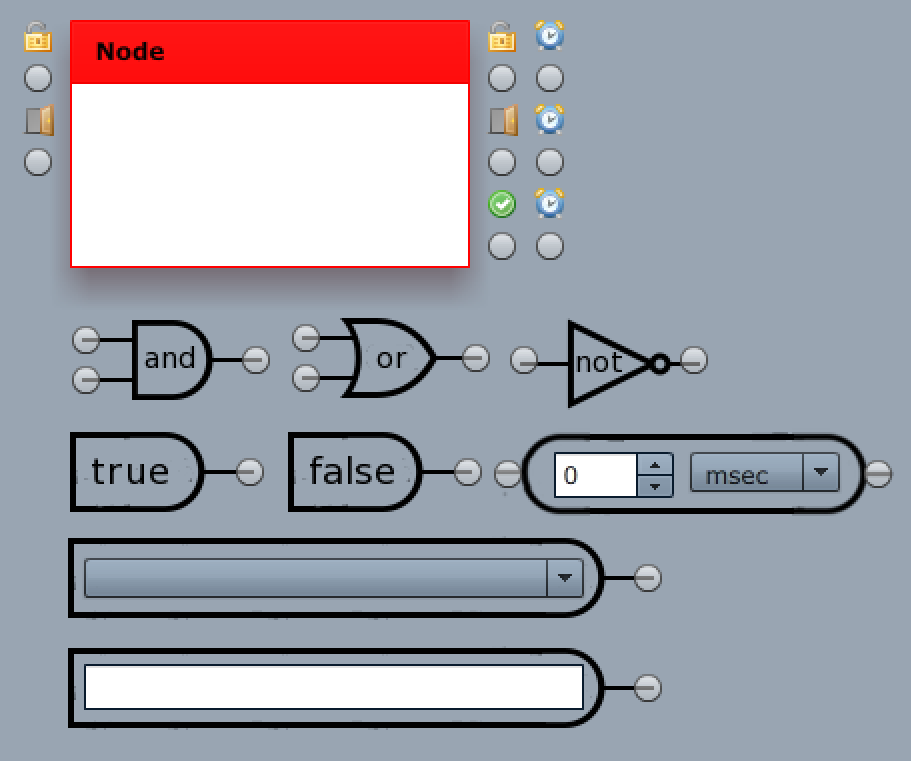
\includegraphics[width=0.38\textwidth]{SyntactischeVormen}
    \caption{Bouwblokken in de story editor.}
    \label{fig:syntactischevormen}
\end{wrapfigure}

Volgens formalisme kan een narratief uitgedrukt worden in syntactische vormen. Deze hebben verder geen waarde of betekenis, totdat er een interpretatie op losgelaten wordt. Een goed voorbeeld hiervan is terug te zien in de wiskunde. 

Zo bestaat de stelling van Pythagoras ook uit syntactische vormen die weergeven worden als letters:

\[ a^2 + b^2 = c^2 \]

Binnen de wiskunde hebben deze letters volgens het formalisme zelf geen betekenis. Dit wordt onderbouwd door het feit dat letters gebruikt kunnen worden voor andere stellingen, functies en vergelijkingen. De interpretatie op de eigenschappen van letter, zoals positie binnen de stelling, geven betekenis aan deze syntactische vorm.

Dit begrip komt ook terug in de editors in de vorm van nodes. Met deze nodes wordt er een narratief geformuleerd die de richtlijnen van het formalisme respecteert. We kunnen ook wel zeggen dat deze syntactische vormen bouwblokken zijn in de editors. In \autoref{fig:syntactischevormen} zijn enkele bouwblokken die in de story editor voorkomen te zien.

\section{Formalisme binnen de story- en dialog editor}
De story- en dialog editor maken beide gebuikt van een ander formalisme. Dit is duidelijk te zien aan hoe het narratief representeert wordt door de editors (zie \autoref{fig:storyeditorvisualisationofstorydata} en \autoref{fig:dialogeditorvisualisationofstorydata}). 

% \begin{figure}
%     \centering
%     \begin{minipage}{.45\textwidth}
%         \centering
%         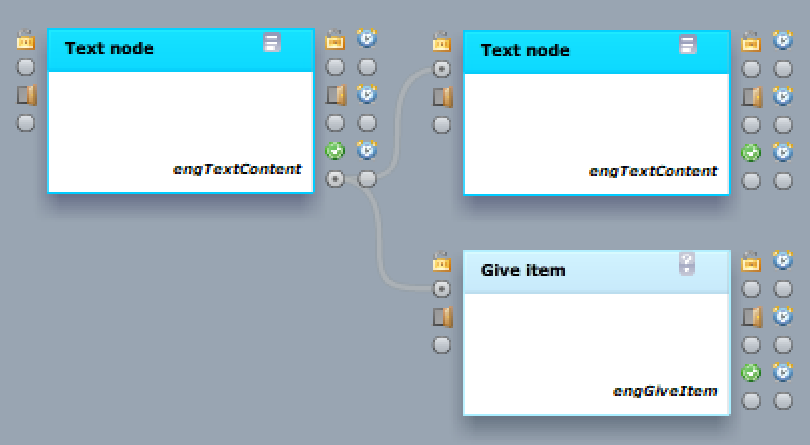
\includegraphics[height=0.4\linewidth]{StoryEditorVisualisationOfStoryData}
%         \caption{Story editor visualisatie van achterliggende data.}
%         \label{fig:storyeditorvisualisationofstorydata}
%     \end{minipage}%
%     \begin{minipage}{.45\textwidth}
%         \centering
%         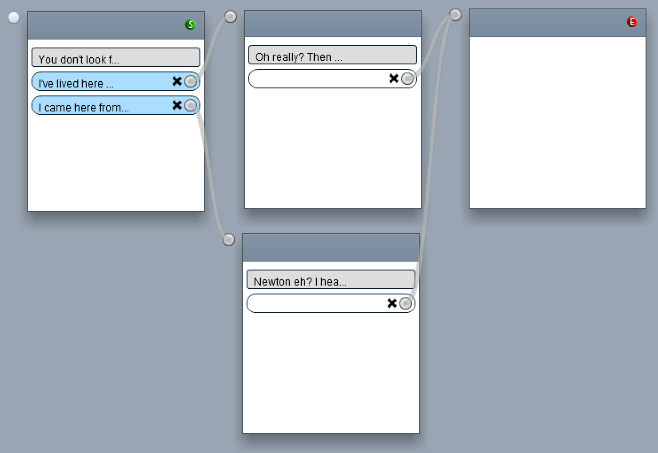
\includegraphics[height=0.4\linewidth]{DialogEditorVisualisationOfStoryData}
%         \caption{Dialog editor visualisatie van achterliggende data.}
%         \label{fig:dialogeditorvisualisationofstorydata}
%     \end{minipage}
% \end{figure}

\begin{figure}[htb]
    \centering
    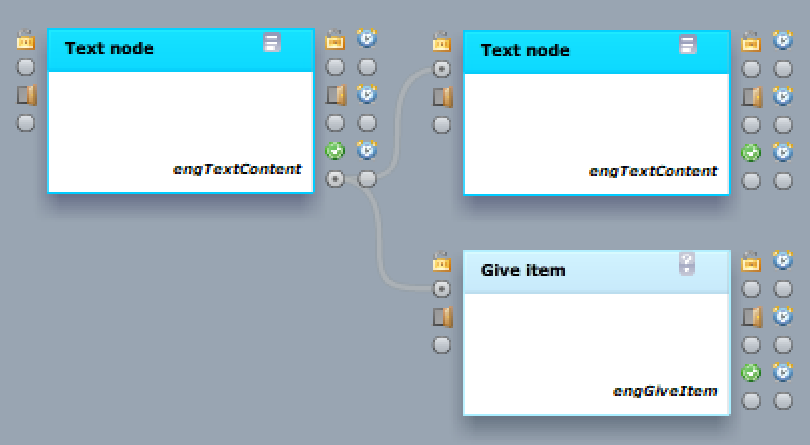
\includegraphics[width=0.45\textwidth]{StoryEditorVisualisationOfStoryData}
    \caption{Story editor visualisatie van achterliggende data.}
    \label{fig:storyeditorvisualisationofstorydata}
\end{figure}

\begin{figure}[htb]
    \centering
    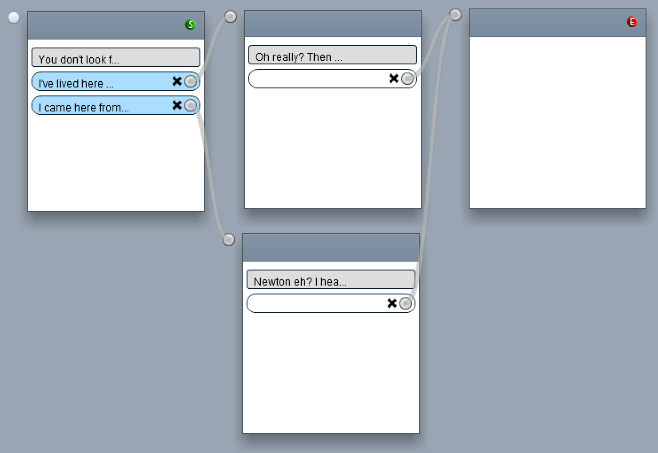
\includegraphics[width=0.45\textwidth]{DialogEditorVisualisationOfStoryData}
    \caption{Dialog editor visualisatie van achterliggende data.}
    \label{fig:dialogeditorvisualisationofstorydata}
\end{figure}

Aan de huidige code base is te zien dat er een nauwe koppeling bestaat tussen de interface en het achterliggende formalisme. Dit maakt het lastig om meerdere formalismen te ondersteunen.

Dit kan een reden zijn geweest waarom er twee editors zijn opgezet; om de scheiding te maken tussen formalismen. Het is een uitdaging om in één omgeving meerdere formalismen te ondersteunen, omdat deze bestaat uit andere syntactische vormen en gebruik maken van andere principes.

Wel is het wenselijk om meerdere formalismen in één omgeving te ondersteunen om de volgende voorkomende problemen op te kunnen lossen:

\begin{itemize}
    \item Houdbaarheid; er hoeft nog maar één omgeving onderhouden te worden in plaats van twee wat schilt in kosten.
    \item Houdbaarheid; generieke editor functionaliteit (copy/ paste, verplaatsen van nodes) kan worden hergebruikt en hoeft maar één keer geïmplementeerd te worden.
    \item Future proofing; benodigde formalismen kunnen in de toekomst worden toegevoegd. Er hoeft niet nog een nieuwe editor gemaakt te worden.
    \item Co-creatie; er zou eventueel een versimpeld formalisme toegevoegd kunnen worden waar klanten mee overweg kunnen. Hiernaast kan het versimpelde formalisme gebruikt worden om de volledige flow van het verhaal in kaart te brengen. Bij \&ranj is er al onderzoek gedaan naar formalisme voor klant co-creatie \cite{Schipper2015}.
\end{itemize}

\section{De scheiding leggen tussen de editor en formalisme}
Om een flexibele tool op te zetten voor het vertellen van diverse digitale interactieve verhalen is het nodig om verschillende formalisme voor diverse doeleinden te kunnen gebruiken. Met de toekomst blik van \&ranj en het ‘bad news’ dialoog moet er een formalisme ondersteund worden waarin een meer AI-benadering toegepast kan worden. Om dit mogelijk te maken moet er een manier komen om formalismen toe te kunnen voegen aan de editors.

Om de scheiding te leggen tussen de editor en het achter liggende formalisme zijn de volgende vragen opgesteld:

\begin{itemize}
    \item Hoe kunnen er bouwblokken worden geformuleerd per formalisme?
    \item Hoe kunnen er regels worden opgelegd aan het verbinden en het in elkaar voegen van deze bouwblokken?
    \item Hoe zou een algoritme eruitzien om vanuit een visuele structuur te compileren naar een formalisme?
\end{itemize}

\subsection{Het formuleren van bouwblokken}
Ieder formalisme wordt ondersteund door syntactische vormen. Een concretere naam die aansluit bij de editors hiervoor is ‘bouwblokken’. Gebruikers van de editors zullen deze bouwblokken gebruiken om een narratief te definiëren volgens een vooraf vastgesteld formalisme. De representatie en interpretatie van deze bouwblokken verschillen dan ook per formalisme. Maar voor de editors zijn het allemaal ‘nodes’ (met eventuele porten) waarmee de node verbonden kan worden aan andere nodes; voor de editor hebben deze nodes geen verdere waarde noch betekenis. Als programmeur moet het mogelijk zijn om op een makkelijke manier bouwblokken te kunnen formuleren. Voor deze use case zijn de volgende requirements opgesteld:

\begin{enumerate}
    \item Ieder formalisme moet onderbouwd worden door een set aan bouwblokken, zodat de gebruiker deze kan gebruiken om binnen de richtlijnen van het formalisme te werken.
    \item Het constructie proces van de bouwblokken moet losstaan van de representatie, zodat verschillende representaties gebruikt kunnen worden voor diverse doeleinden.
    \item De representatie van deze bouwblokken moeten losgekoppeld worden van enige waarde of betekenis, zodat deze later volgens het formalisme geïnterpreteerd kunnen worden.
\end{enumerate}

De voornaamste manier om een node te construeren is om de bijbehorende klasse te instantiëren. Dit geeft ons een node object waarvan de representatie statisch is; het instantiëren van de node klassen resulteert altijd in hetzelfde object. Dit schendt requirements 2 en 3. Om constructie van representatie los te koppelen, en zo te voldoen aan de tweede requirement, kunnen er parameters de constructor van de node klasse gedefinieerd worden die de eigenschappen en representatie van de node beschrijven. In \autoref{fig:storyeditorvisualisationofstorydata} is een van de bouwblokken in het formalisme van de story editor terug te zien: de ContentTypeNode. Dit bouwblok heeft een label en 8 porten. Het zojuist beschreven constructie proces voor deze node zou er als volgt uit kunnen zien:\\


\noindent\fbox{
    \parbox{\textwidth}{
        \textbf{Functie handtekening}
constructor Node(label: string, markup: string, allowBodyConnections: boolean, ports: Port[]): Node

\textbf{Voorbeeld}
new Node(‘ContentType’, ‘<rect class=”node-body” width=”100” height=”100”><text/></rect>’, false, [new Port(…), new Port(…), …]);
    }
}